\cleardoublepage
\newpage
\ifdefined\EnableIncludeImages
    \ThisULCornerWallPaper{1.0}{chapterimage.eps}
\fi
\chapter*{Introdução} % 
\addcontentsline{toc}{chapter}{Introdução} %% Agregando manualmente a la tabla de contenidos

%% Usei a mesma estrutura do inicio do quijote
No meu querido povoado de Occo, na época da minha primeira década, eu passava os dias dividindo meu tempo entre os trabalhos da chacra\footnote{Também escrita como \textit{chakra}, esta é uma palavra quéchua que faz referência a um terreno de cultivo.}, meus jogos infantis e inumeráveis passeios pelo campo.
Os trabalhos da chacra, mesmo que fossem pesados para mim, eram possíveis de serem feitos porque estavam divididos com toda a família.
Contudo, os dias no campo não transcorriam limpos de surpresas, dado que, de tempo em tempo, algum de nossos animais se perdia; nesses casos, eu saía pelas ladeiras dos montes chamando-os pelo seu nome até que escutava uma resposta, geralmente em forma de um lamento cheio de saudade.
Essa tática era especialmente eficaz com meu burrinho, pois ele conseguia escutar meu chamado mesmo estando em outras montanhas. Assim, quando eu gritava seu nome, ele voltava a mim gritando e chorando, escolhendo seu caminho em função da direção da minha voz.
Em outras ocasiões, percebíamos que desapareciam animais pequenos, como frangos ou porquinhos-da-índia; porém, após observar as evidências e fazer um trabalho ``detetivesco'', descobríamos que sua ausência era devido à ``visita'' de algum falcão, zorro ou gato-do-mato.
Nesses casos, nós só podíamos chorar por eles; contudo, poucas eram as vezes que perdíamos animais dessa forma, dado que, além das pessoas da casa, nós tínhamos animais como cachorros e gatos que nos ajudavam a vigiar.

\ifdefined\EnableIncludeImages
\begin{wrapfigure}{r}{0.49\textwidth}
  \begin{center}
  \vspace{-20pt}
    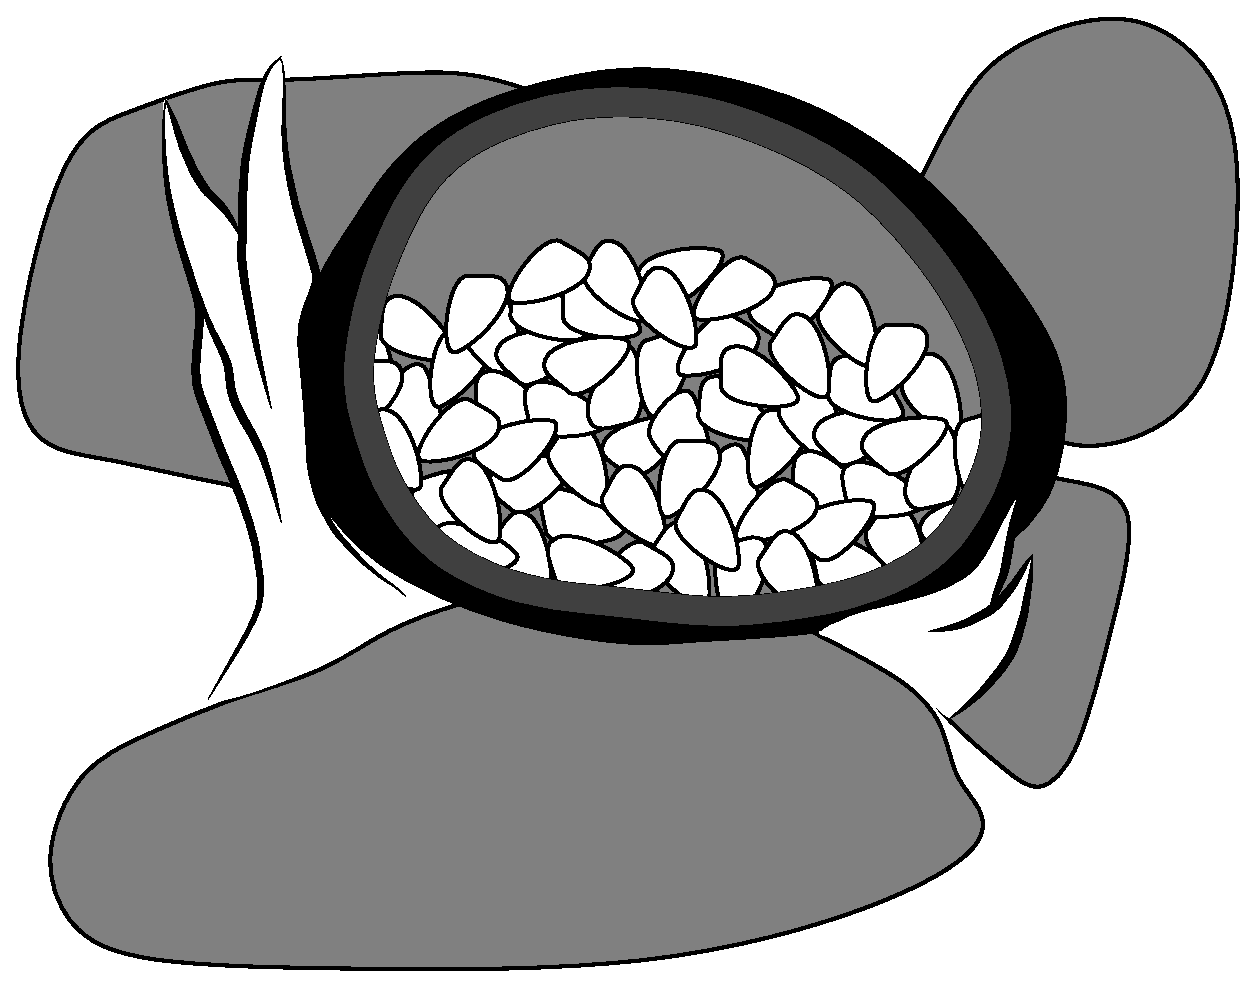
\includegraphics[width=0.47\textwidth]{cancha.eps}
  \end{center}
  \vspace{-20pt}
  %\caption{Zandor}
\end{wrapfigure}
\fi
Minha família não era endinheirada, e talvez esse conceito escapava a meu entendimento naquela época, mas nada do que realmente importava me faltava.
Lembro-me de que minha casa era de adobe e madeira, com teto de telha, e minha mãe cozinhava nossos alimentos sobre uma fogueira pequena. Minhas irmãs e eu, com muita frequência, usávamos roupas que, a simples vista, qualquer pessoa consideraria que eram várias medidas menores ou maiores das que realmente precisávamos;
porém, para mim e minhas irmãs, isso não importava. Minha casa era um castelo amplo e fresco no qual eu ia descansar após voltar da escola ou do trabalho na chacra. 
A comida da minha mãe era o melhor do dia, pois estava cheia dos sabores dos produtos que nós mesmos cultivávamos ou cuidávamos. 
Em dias especiais, meu pai ia ao rio para pescar e comíamos peixe frito no almoço. Outras vezes, na estação seca, comíamos charque\footnote{Carne desidratada ao sol.} com alguma mistura de ovos de perdiz ou de galinha, dependendo da sorte do dia.
O queijo e o leite não faltavam nas nossas refeições, que tanto podiam ser de cabra ou de vaca.
As sobremesas dependiam da estação do ano, pois as frutas como figos-da-índia, pêssego, figo, sanky\footnote{Fruta dos Andes peruanos com múltiplos benefícios para a saúde.}, entre outras, tinham cada uma sua temporada. Também havia épocas para sobremesas elaboradas com milho fresco e outras com chila-caiota; com este último, minha mãe fazia meu mingau favorito. Era inacreditável para mim que um creme de semelhante majestade pudesse ser preparado com só um pouco de doce de molle\footnote{O \textit{molle} ou \textit{Lithraea molleoides}, é um substituto do açúcar.}, canela, cravo e chila-caiota\footnote{Chila-caiota ou \textit{Cucurbita ficifolia}.}.

Minhas irmãs e eu gostávamos de brincar juntos, sair para passear procurando frutas e ir apreciar aos animais silvestres. Em geral, nós não tínhamos discussões importantes; porém, devo reconhecer que eu, de tempo em tempo, acostumava fazer-lhes alguma travessura.
Nesses casos, elas recorriam às maiores autoridades da casa, com os senhores que governavam e decidiam sobre o bem e o mal, ou seja, meus pais. 
Lembro-me de que, no princípio, meu pai me falava com frases como:\\\indent
---Aule, você não deve esconder a boneca da sua irmã.\\\indent
Se o assunto era mais grave, ele dizia: \\\indent
---Aurelio! Por que você colocou um grilo na cabeça da sua irmã?\\\indent
Se minha insistência na procura de problemas chegava a níveis maiores, meu pai gritava com energia:\\\indent
---Aulicha! Por que você colocou pimenta na balinha da sua irmã?\\\indent
Assim, quando eu escutava meu pai me chamar de \textit{Aulicha}, eu já sabia que minha sorte tinha sido decidida e que uma chicotada estava próxima. A ideia de fugir sempre passava por minha cabeça; porém, minhas experiências anteriores me indicavam que isso só iria me prejudicar mais e ia resignado diante do meu pai. Inclusive, em várias ocasiões, ele me pedia para lhe alcançar aquele chicote de três pontas, pequeno e veloz, que era ao mesmo tempo um velho conhecido e meu principal antagonista.
Porém, após a punição e depois de algum tempo, cerca de meia hora,
ele me procurava para me consolar e me abraçando dizia:\\\indent
---Por que você se comporta assim? Você não deve incomodar a sua irmã ... comporte-se melhor.


A minha vida no campo sempre estava cheia de contrapontos, tantos eram os momentos tristes quanto os alegres, e algumas vezes, mais das que me permitiriam pensar que era só uma casualidade, os momentos tristes preparavam um caminho inevitável e irreversível às épocas alegres e vice-versa; como um ciclo que se retroalimenta para se manter perpétuo. 
Assim, uma das minhas maiores alegrias era saber que meu pai retornava de viagem, geralmente da costa do Peru, não só devido à saudade que deixava a partida dele e a alegria que trazia seu retorno, mas também porque ele voltava cheio de presentes. 
Nos trazia doces, bolachas, brinquedos, roupas, entre outros, aos quais, comumente, nós nos Andes não tínhamos acesso.
Por outro lado, entre meus momentos mais tristes, estava a perda de algum ente querido e a consequente impotência ao não ser capaz de evitar sua partida. 
No entanto, tudo isso é parte da vida e gostaria compartilhar com vocês alguns desses momentos.



%Ayacucho é uma cidade do distrito de Ayacucho, na província de Huamanga, no departamento de Ayacucho, no Peru
